\chapter{Uczenie modelu detekcji choroby Alzheimera oraz jego wykorzystanie}

W tej pracy chcę przedstawić możliwości wykorzystania bibliotek uczenia maszynowego w środowisku \emph{.NET} w celu uczenia oraz późniejszego wykorzystania modelu głębokiej sieci neuronowej do detekcji choroby Alzheimera oraz stopnia demencji na obrazach rezonansu magnetycznego mózgów pacjentów, a także postaram się je porównać między sobą oraz z istniejącymi rozwiązaniami także spoza środowiska \emph{.NET}.

\section{Zbiór danych}

Wykorzystany zbiór pochodzi z platformy Kaggle (udostępniony jest pod adresem \url{www.kaggle.com/datasets/tourist55/alzheimers-dataset-4-class-of-images} na licencji \emph{Open Data Commons Open Database License} (\emph{ODbL}) wersji $1.0$) \cite{kaggle-alzheimers-dataset}.
Jest wstępnie podzielony na zbiór treningowy oraz testowy w celu zapewnienia powtarzalności i porównywalności wyników uzyskanych z użyciem różnych narzędzi i z różnych źródeł.
Zawiera on zestaw obrazów uzyskanych z badań rezonansem magnetycznym (MRI), których celem jest analiza i diagnoza otępienia spowodowanego chorobą Alzheimera.
Obrazy te są dwuwymiarowym wycinkiem trójwymiarowego skanu rezonansu magnetycznego mózgu, który najlepiej obrazuje strukturę mózgu i potencjalne zmiany chorobowe.
Mają wymiary $208 \times 176$ pikseli -- wystarczająco duże, aby widoczne były nawet drobne detale ale na tyle małe, aby były możliwe do przetworzenia przez mniejsze sieci neuronowe a także umożliwiły ich znacznie szybsze szkolenie.

Zbiór danych składa się z czterech kategorii obrazów, zarówno w zbiorze treningowym, jak i testowym:

\begin{itemize}

  \item
        Brak demencji (\emph{Non Demented}) -- ta kategoria zawiera obrazy mózgów osób niebędących dotkniętymi demencją.
        W zbiorze treningowym znajduje się 2560 obrazów, a w zbiorze testowym 640 obrazów, co daje sumarycznie 3200 zdjęć z tej kategorii.

  \item
        Bardzo łagodna demencja (\emph{Very Mild Demented}) -- zbiór ten obejmuje obrazy osób z bardzo łagodnym stopniem demencji.
        W zbiorze treningowym znajduje się 1792 obrazy, a w zbiorze testowym 448 obrazów, co daje łącznie 2240 obrazów z tej kategorii.

  \item
        Łagodna demencja (\emph{Mild Demented}) -- ten zbiór zawiera obrazy mózgów pacjentów cierpiących na łagodne otępienie związanego z chorobą Alzheimera.
        W zbiorze treningowym znajduje się 717 obrazów, a w zbiorze testowym 179 obrazów, co daje łączną sumę 896 obrazów z tej kategorii.

  \item
        Umiarkowana demencja (\emph{Moderate Demented}) -- ta kategoria obejmuje obrazy mózgów pacjentów już z wyższym stopniem demencji związanym z chorobią Alzheimera.
        W zbiorze treningowym znajduje się 52 obrazy, a w zbiorze testowym 12 obrazów, co daje łącznie 64 obrazy z tej kategorii.

\end{itemize}

\begin{figure}[ht]
  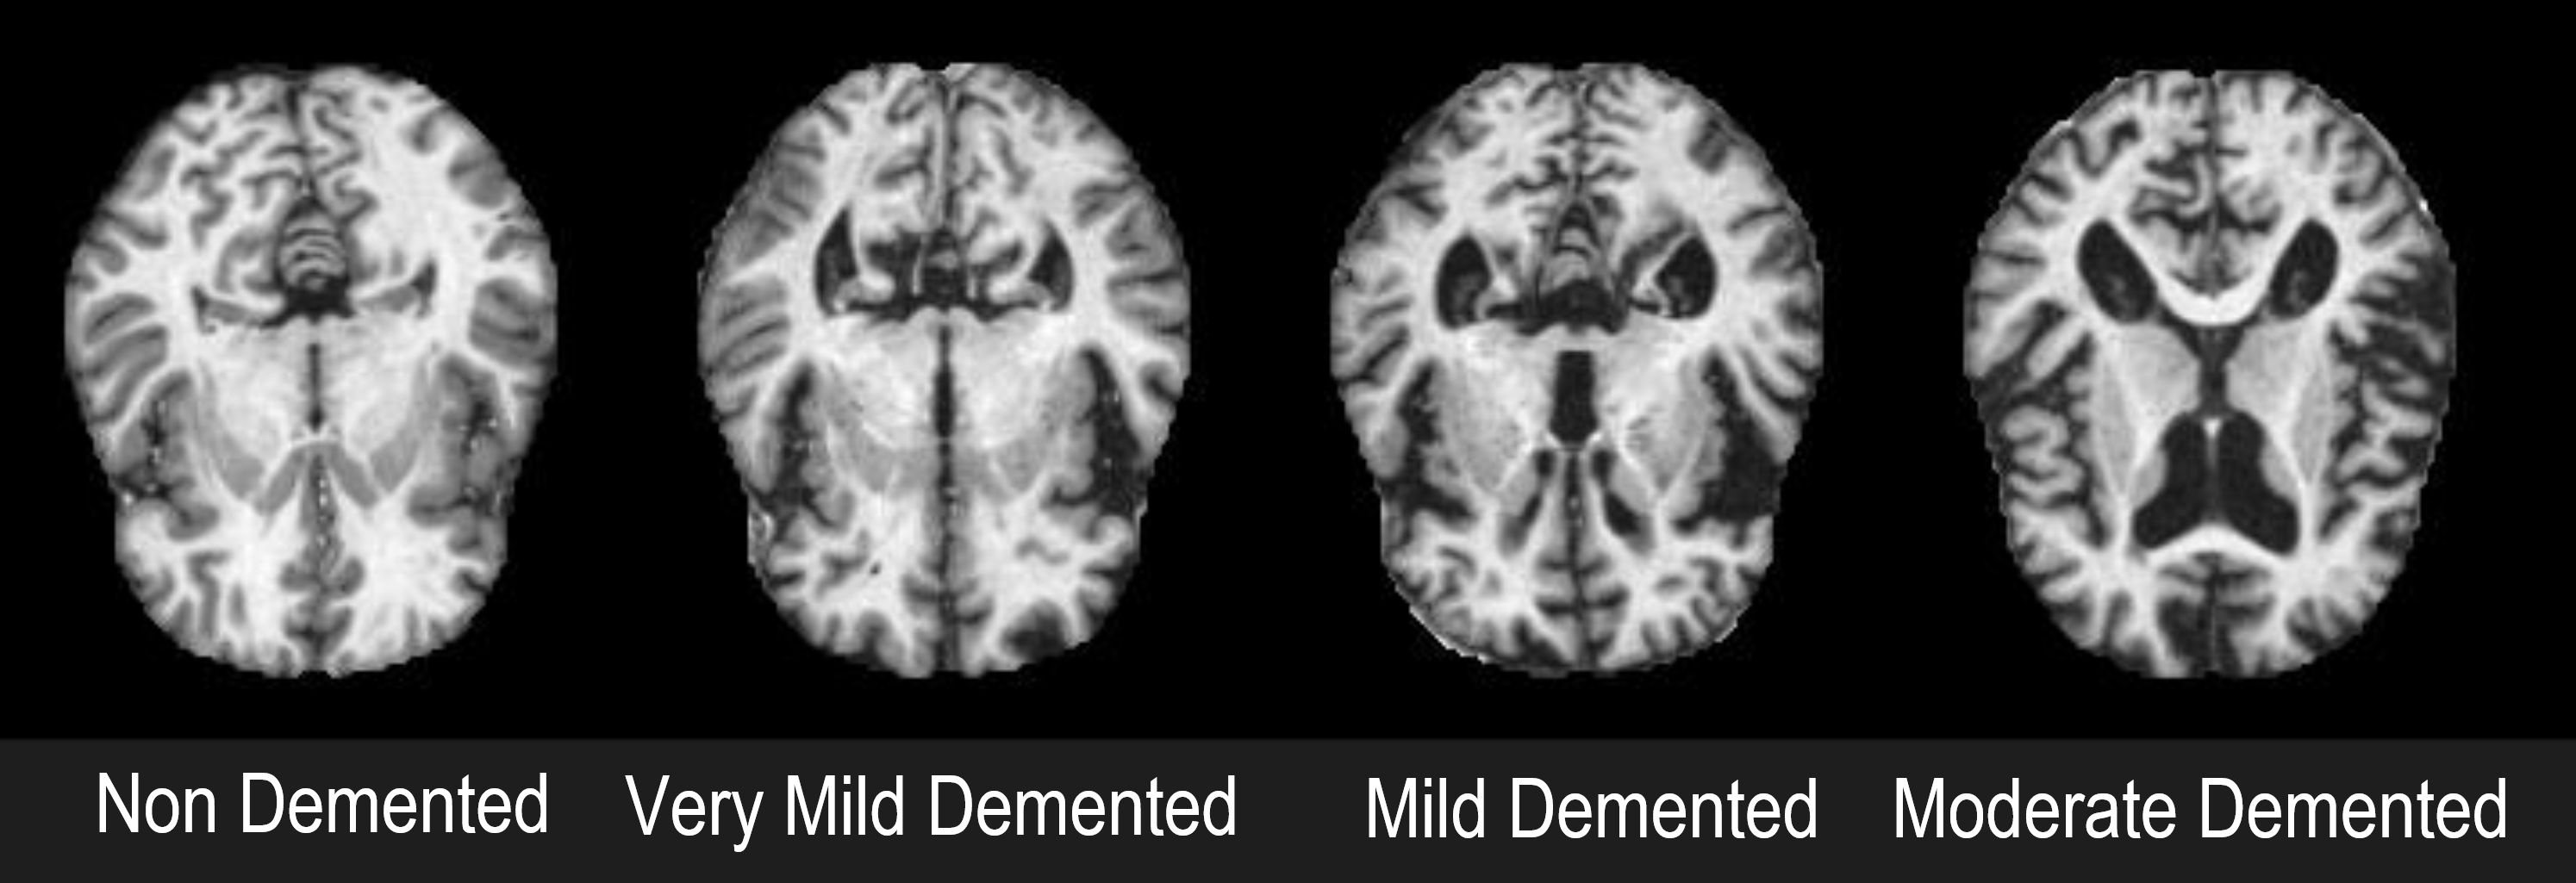
\includegraphics[width=\textwidth]{dataset-image-examples}
  \caption[Zestawienie przykładowych obrazów z każdej kategorii zbioru danych]{Zestawienie przykładowych obrazów z każdej kategorii zbioru danych \cite{kaggle-alzheimers-dataset}, gdzie przedstawione od lewej są: obraz mózgu osoby bez demencji, obraz mózgu osoby z bardzo lekką demencją, obraz mózgu osoby z lekką demencją o podłożach w chorobie Alzheimera oraz obraz mózgu osoby z umiarkowaną demencją chorą na Alzheimera.}
  \label{fig:dataset-image-examples}
\end{figure}

Przykłady obrazów z poszczególnych kategorii przedstawione są na \hyperref[fig:dataset-image-examples]{rysunku \ref*{fig:dataset-image-examples}}.

\section{Uczenie modelu z użyciem narzędzia ML.NET}

\subsection{Uczenie modelu z użyciem narzędzia ML.NET Model Builder}

\subsection{Uczenie modelu z wykorzystaniem niestandardowego kodu biblioteki ML.NET}

\section{Uczenie niestandardowego modelu z użyciem biblioteki TenserFlow.NET}

Opis procesu uczenia modelu z użyciem biblioteki TenserFlow.NET

\section{Porównanie wyników}

Przedstawienie wyników uzyskanych z użyciem wszystkich narzędzi narzędzi

\section{Wykorzystanie modelu w aplikacji z użyciem biblioteki ML.NET}

W jaki sposób wykorzystać można model w aplikacji
